\chapter{Implementacija i korisničko sučelje}
		
		\section{Korištene tehnologije i alati}
		
			Komunikacija u timu realizirana je korištenjem aplikacije \underline{WhatsApp} \footnote{\href{https://www.whatsapp.com/}{Whatsapp}} za manje i
			kraće dogovore, a za dulje i veće dogovore komunikacija je realizirana korištenjem aplikacije \underline{Microsoft Teams} \footnote{\href{https://www.microsoft.com/hr-hr/microsoft-365/microsoft-teams/group-chat-software}{Microsoft Teams}}. Za izradu UML dijagrama korišten je alat \underline{Astah UML} \footnote{\href{https://astah.net/products/astah-uml/}{Astah UML}}. Kao sustav za upravljanje izvornim kodom Git \footnote{\href{https://git-scm.com/}{Git}}. Udaljeni repozitorij projekta je dostupan na web platformi \underline{GitLab} \footnote{\href{https://www.gitlab.com}{Gitlab}}.

            Kao razvojno okruženje korišten je \underline{Microsoft Visual Studio Code} \footnote{\href{https://code.visualstudio.com/}{Microsoft Visual Studio Code}}. Microsoft Visual Studio Code trenutno je \underline{najpopularnije} \footnote{\href{https://pypl.github.io/IDE.html}{Deset najraširenijih razvojnih okruženja}} razvojno okruženje, iznimno je prilagodljiv raznim potrebama programera i potrebama samog programskog jezika.
            
            Aplikacija je izrađena u dva dijela. Backend dio je napisan koristeći radni okvir \underline{Express.js} \footnote{\href{https://expressjs.com/}{Express.js}} u programskom jeziku \underline{TypeScript} \footnote{\href{https://www.typescriptlang.org/}{TypeScript}}, a frontend dio je napisan koristeći biblioteku \underline{React.js} \footnote{\href{https://reactjs.org/}{React.js}} u programskom jeziku \underline{JavaScript} \footnote{\href{https://www.javascript.com/}{JavaScript}}.
            
            Express.js radni okvir je javno dostupan, besplatan te otvorenog izvora pružen od strane \underline{OpenJS Foundation-a} \footnote{\href{https://openjsf.org/}{OpenJS Foundation}}. Express.js je jednostavna i prilagodljiv \underline{Node.js}\footnote{\href{https://nodejs.org/en/}{Node.js}} radni okvir koja pruža izdržljiv skup značajki za web i mobilne aplikacije.
            
            React.js je JavaScript biblioteka za izradu interaktivnih sučelja unutar web aplikacija. Održavana je od strane Facebooka, a najčešće je korišten kao osnova u razvoju web aplikacija.
            
            Korištena baza podataka je \underline{PostgreSQL} \footnote{\href{https://www.postgresql.org/}{PostgreSQL}}. PostgreSQL je besplatna, objektno-relacijska baza podataka sa više od 30 godina aktivnog razvoja.
            
            Cijela aplikacija poslužena je na \underline{Heroku} \footnote{\href{https://www.heroku.com/home}{Heroku}}. Heroku je platforma koja omogućuje jednostavno i sigurno puštanje  u pogon i nadziranje aplikacija. Konkretno, koristimo dvije Heroku aplikacije, jednu za backend i jednu za frontend te u sklopu backend aplikacije koristimo i jednu instancu PostrgeSQL baze podataka.
			
			\eject 
		
	
		\section{Ispitivanje programskog rješenja}
			
			\textbf{\textit{dio 2. revizije}}\\
			
			 \textit{U ovom poglavlju je potrebno opisati provedbu ispitivanja implementiranih funkcionalnosti na razini komponenti i na razini cijelog sustava s prikazom odabranih ispitnih slučajeva. Studenti trebaju ispitati temeljnu funkcionalnost i rubne uvjete.}
	
			
			\subsection{Ispitivanje komponenti}
			\textit{Potrebno je provesti ispitivanje jedinica (engl. unit testing) nad razredima koji implementiraju temeljne funkcionalnosti. Razraditi \textbf{minimalno 6 ispitnih slučajeva} u kojima će se ispitati redovni slučajevi, rubni uvjeti te izazivanje pogreške (engl. exception throwing). Poželjno je stvoriti i ispitni slučaj koji koristi funkcionalnosti koje nisu implementirane. Potrebno je priložiti izvorni kôd svih ispitnih slučajeva te prikaz rezultata izvođenja ispita u razvojnom okruženju (prolaz/pad ispita). }
			
			
			
			\subsection{Ispitivanje sustava}
			
			 \textit{Potrebno je provesti i opisati ispitivanje sustava koristeći radni okvir Selenium\footnote{\url{https://www.seleniumhq.org/}}. Razraditi \textbf{minimalno 4 ispitna slučaja} u kojima će se ispitati redovni slučajevi, rubni uvjeti te poziv funkcionalnosti koja nije implementirana/izaziva pogrešku kako bi se vidjelo na koji način sustav reagira kada nešto nije u potpunosti ostvareno. Ispitni slučaj se treba sastojati od ulaza (npr. korisničko ime i lozinka), očekivanog izlaza ili rezultata, koraka ispitivanja i dobivenog izlaza ili rezultata.\\ }
			 
			 \textit{Izradu ispitnih slučajeva pomoću radnog okvira Selenium moguće je provesti pomoću jednog od sljedeća dva alata:}
			 \begin{itemize}
			 	\item \textit{dodatak za preglednik \textbf{Selenium IDE} - snimanje korisnikovih akcija radi automatskog ponavljanja ispita	}
			 	\item \textit{\textbf{Selenium WebDriver} - podrška za pisanje ispita u jezicima Java, C\#, PHP koristeći posebno programsko sučelje.}
			 \end{itemize}
		 	\textit{Detalji o korištenju alata Selenium bit će prikazani na posebnom predavanju tijekom semestra.}
			
			\eject 
		
		
		\section{Dijagram razmještaja}
			
			
			 \textit{Dijagram razmještaja koristi se za prikaz topologije sustava pri čemu je naglasak stavljen na odnose između sklopovskih i programskih komponenti. Oni opisuju korištenu programsku potporu sustava te njegove elemente i okolinu izvođenja. Osnovni su elementi čvorovi, artefakti te spojevi koji predstavljaju komunikacijske puteve između njih. }
			 
			 \textit{Klijent putem svojeg web preglednika pristupa web aplikaciji koja se vrti na cloud serveru. Sva komunikacija odvija se putem protokola HTTP. Na poslužiteljskom računalu nalaze se baza podataka te aplikacija.}
			 \begin{figure}[H]
    			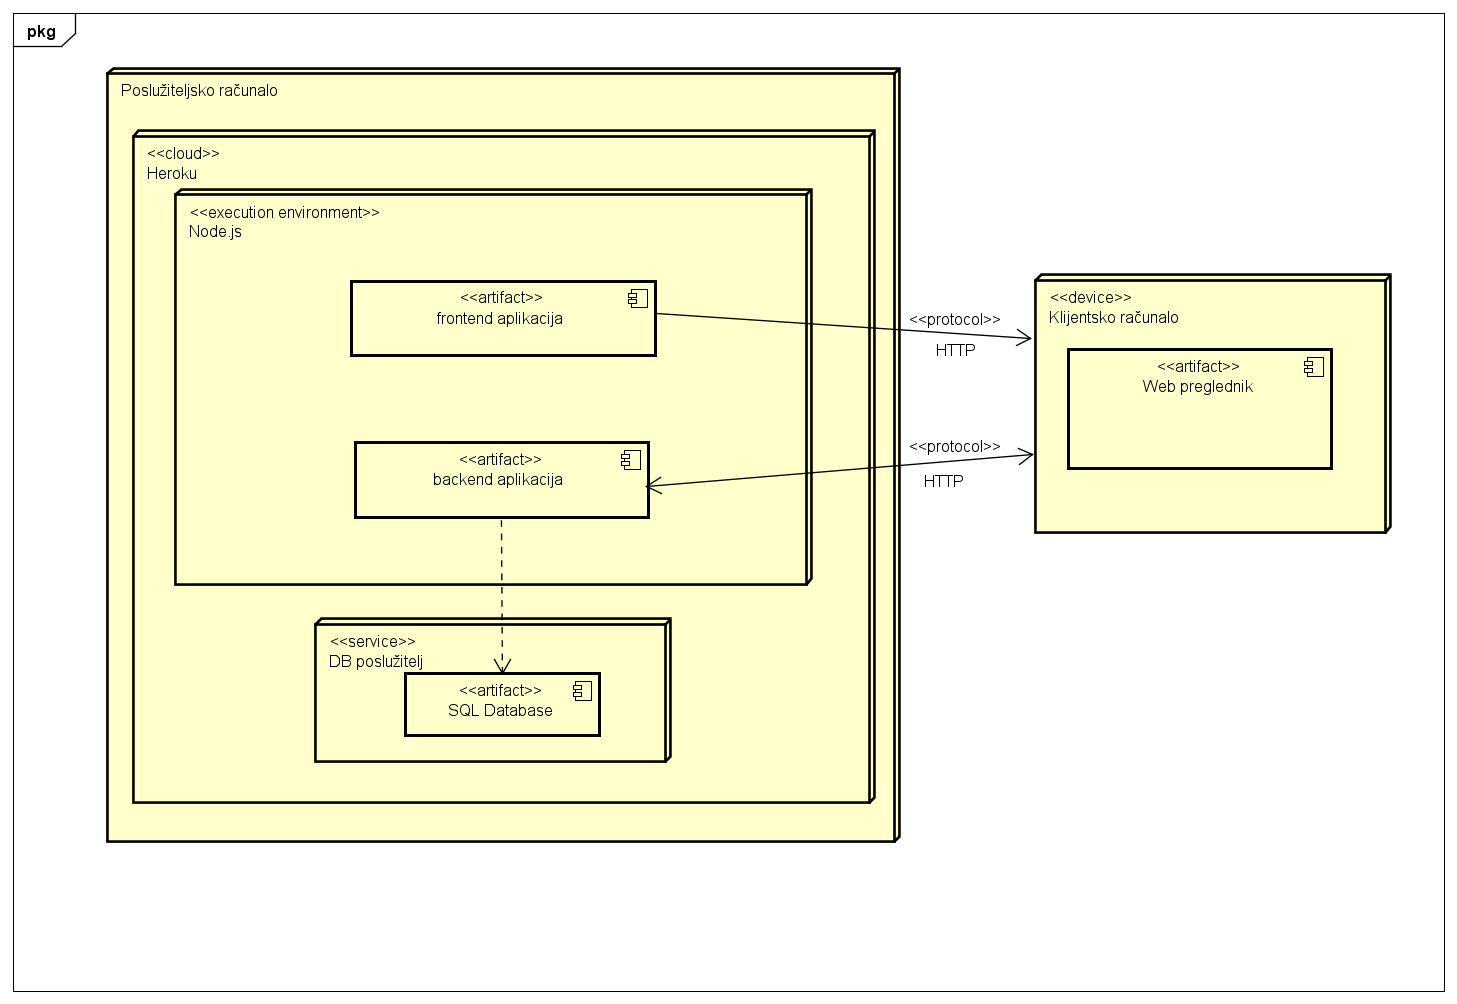
\includegraphics[width=1\linewidth]{dijagrami/Deployment Diagram.png}
    			\caption{Dijagram razmještaja}
    			\label{fig:Dijagram razmještaja} 
    		\end{figure}
			\eject 
		
		\section{Upute za puštanje u pogon}
		
		    Prije ikakve radnje, potrebno je klonirati \textit{GitLab} repozitorij sa kodom te otvoriti terminal (i opcionalno sistemski preglednik) u tom direktoriju. Udaljeni \textit{GitLab} repozitorij možete pronaći na  \underline{\href{https://gitlab.com/Cubi5/seven}{ovoj poveznici}}
		    
		    Kako bi kloniranje bilo moguće potrebno je imati instalirani \textit{Git} klijent na računalu. \textit{Git} klijent moguće je preuzeti na \underline{\href{https://git-scm.com/downloads}{ovoj poveznici}}.
		    
		    Još jedan uvjet kako bi aplikacija radila lokalno jest instaliran \textit{Node.js}. \textit{Node.js} moguće je preuzeti na \underline{\href{https://nodejs.org/en/download/}{ovoj poveznici}}. Instalacijom \textit{Node.js} aplikacije, instalirat će vam se i \textit{\underline{npm}} \footnote{\href{https://www.npmjs.com/}{npm}} koji je zapravo abrevijacija od \textit{Node Package Manager}. Samo ime govori da je to alat za upravljanje \textit{Node.js} paketima.

		        
				\pagebreak
		

				\subsection{Frontend aplikacija}
	        
						\subsubsection*{Lokalna instalacija}
	        
	          		Da bismo pokrenuli lokalnu frontend aplikaciju potrebno je unutar terminala pozicionirati se u frontend mapu unutar korijenskog direktorija. 
	            
								\begin{center}
										\texttt{cd frontend}
								\end{center}
								
								Sada je potrebno instalirati potrebne pakete za uspješan rad aplikacije. To činimo pokretanjem naredbe
								
								\begin{center}
										\texttt{npm install}
								\end{center}
								
								Nakon instalacije paketa, potrebno je podesiti i lokalni \textit{host} file. Da bismo uredili \textit{host} file prvo ga je potrebno locirati, a sama lokacija ovisi o operacijskom sustavu. Ukoliko koristimo operacijski sustav na bazi \textit{Linuxa} \textit{host} file se nalazi na lokaciji \texttt{/etc/hosts}, dok se na \textit{Windows} operacijskom sustavu ta datoteka nalazi na \verb$C:\Windows\System32\drivers\etc\hosts$
								
								Jednom kada smo je locirali, potrebno je na kraj datoteke dodati redak

								\begin{center}
										\texttt{127.0.0.1	frontend-local.parkirajme.xyz}
								\end{center}
								
								Dodavanjem ovog retka, završili smo lokalnu instalaciju servera te server možemo pokrenuti naredbom
								
								\begin{center}
										\texttt{npm run dev}
								\end{center}
								
								Kako bi sve ispravno radilo lokalnom serveru ćemo pristupiti sa sljedeće adrese

								\begin{center}
										\href{http://frontend-local.parkirajme.xyz:3000/}{\texttt{frontend-local.parkirajme.xyz:3000}}
								\end{center}
		             
						\pagebreak
		    
						\subsubsection*{Heroku instalacija}
	        
								Kako bismo frontend aplikaciju pustili u pogon, potrebne je kreirati novu aplikaciji na Heroku platformi.
								
								\begin{enumerate}
									\item Otvoriti \href{https://dashboard.heroku.com/apps}{heroku.com} stranicu i prijaviti se ukoliko to već nismo prethodno učinili.
									\item U gornjem desnom kutu možemo vidjeti gumb \textit{New} te kada ga pritisnemo otvara nam se padajuća lista i u njoj odabiremo \textit{Create new app}
									\item Otvara nam se forma za kreiranje nove aplikacije te tu navodimo ime aplikacije koje može biti proizvoljno. Također na tom koraku odabiremo i regiju servera i tu je poželjno postaviti server koji je nama najbliži, a to je Europa.
									\item Pritiskom na \textit{Create app} stvaramo aplikaciju
		        		\end{enumerate}
		        
		        		Sada kada je Heroku aplikacija napravljena potrebno je otvoriti \texttt{.git/config} datoteku unutar korijenskog direktorija aplikacije te na kraj te datoteke potrebno je dodati

                \begin{verbatim}
    [remote "heroku-frontend"]
        	url = https://git.heroku.com/${imeHerokuAplikacije}.git
        	fetch = +refs/heads/*:refs/remotes/heroku-frontend/*
								\end{verbatim}
								
								te umjesto \texttt{\{imeHerokuAplikacije\}} potrebno je umetnuti ime novostvorene aplikacije. Kada smo podesili \texttt{config} datoteku sve što je potrebno napraviti je pozicionirati se u direktorij frontend aplikacije te iz terminala pokrenuti 

								\begin{center}
										\texttt{npm run deploy}
								\end{center}
								
								Nakon par minuta aplikacija će biti puštena u pogon.

						\pagebreak
						
						\subsection{Backend aplikacija}
	        
						\subsubsection*{Lokalna instalacija}
	        
	          		Da bismo pokrenulni lokalnu backend aplikaciju potrebno je unutar terminala pozicionirati se u backend mapu unutar korijenskog direktorija. 
	            
								\begin{center}
										\texttt{cd backend}
								\end{center}
								
								Sada je potrebno instalirati potrebne pakete za uspješan rad aplikacije. To činimo pokretanjem naredbe
								
								\begin{center}
										\texttt{npm install}
								\end{center}
								
								Nakon instalacije paketa, završili smo lokalnu instalaciju servera te server možemo pokrenuti naredbom
								
								\begin{center}
										\texttt{npm run dev}
								\end{center}
								
								Sada je server pokrenut te mu možemo pristupiti koristeći naredbeni redak i naredbu \texttt{curl} ili pak neki drugi alat za kreiranje HTTP zahtjeve poput alata \underline{Postman} \footnote{\href{https://www.postman.com/}{Postman}}.
		             
						\pagebreak
		    
						\subsubsection*{Heroku instalacija}
	        
								Kako bismo backend aplikaciju pustili u pogon, potrebno je kreirati novu aplikaciji na Heroku platformi.
								
								\begin{enumerate}
									\item Otvoriti \href{https://dashboard.heroku.com/apps}{heroku.com} stranicu i prijaviti se ukoliko to već nismo prethodno učinili.
									\item U gornjem desnom kutu možemo vidjeti gumb \textit{New} te kada ga pritisnemo otvara nam se padajuća lista i u njoj odabiremo \textit{Create new app}
									\item Otvara nam se forma za kreiranje nove aplikacije te tu navodimo ime aplikacije koje može biti proizvoljno. Također na tom koraku odabiremo i regiju servera i tu je poželjno postaviti server koji je nama najbliži, a to je Europa.
									\item Pritiskom na \textit{Create app} stvaramo aplikaciju
		        		\end{enumerate}
		        
		        		Sada kada je Heroku aplikacija napravljena potrebno je otvoriti \texttt{.git/config} datoteku unutar korijenskog direktorija aplikacije te na kraj te datoteke potrebno je dodati

                \begin{verbatim}
    [remote "heroku-backend"]
        	url = https://git.heroku.com/${imeHerokuAplikacije}.git
        	fetch = +refs/heads/*:refs/remotes/heroku-backend/*
								\end{verbatim}
								
								te umjesto \texttt{\{imeHerokuAplikacije\}} potrebno je umetnuti ime novostvorene aplikacije. Kada smo podesili \texttt{config} datoteku sve što je potrebno napraviti je pozicionirati se u direktorij backend aplikacije te iz terminala pokrenuti 

								\begin{center}
										\texttt{npm run deploy}
								\end{center}
								
								Nakon par minuta aplikacija će biti puštena u pogon.
						
						\pagebreak
		    
				\subsection{Baza podataka}
			
						\subsubsection*{Lokalna instalacija}
						
								Potrebno je preuzeti \textit{pgAdmin} aplikaciju uz koju standardno dolazi i \textit{PostgreSQL} server. Pokrenuti instalaciju te uz \textit{pgAdmin} klijenta odabrati i \textit{PostgreSQL} server za instalaciju. Nakon instalacije potrebno je postaviti korisnika. Nakon instalacije \textit{pgAdmin} klijent i sam \textit{PostgreSQL} server su pokrenuti.
								
						\subsubsection*{Lokalna konfiguracija}
								
								Nakon instalacije, potrebno je napraviti novu lokalnu bazu.
								
								\begin{enumerate}
										\item Proširiti \textit{Servers} te, ovisno o preuzetoj verziji \textit{PostgreSQL} servera, proširiti  \textit{PostgreSQL XX}
										\item Desni klik na \textit{Databases} te \textit{Create} te \textit{Database...}
										\item Otvara se modal te kao \textit{Database} vrijednost stavljamo proizvoljni naziv
										\item Odabiremo \textit{Spremi} te time stvaramo novu bazu
								\end{enumerate}
								
								Nakon stvorene baze potrebno je stvoriti konekcijski \textit{connection string}. Njega ćemo stvoriti što ćemo vrijednosti u vitičastim zagradama zamijeniti s pravim vrijednostima.
								
								\begin{center}
										\texttt{postgres://{username}:{password}@{hostname}:{port}/{database}}
								\end{center}
								
								\begin{enumerate}
										\item username - inicijalni username je \textit{postgres}
										\item password - lozinka postavljena prilikom instalacije
										\item hostname - pošto je server lokalni, hostname će biti \textit{localhost}
										\item port - inicijalni priključak PostgreSQL servera je \textit{5432}
										\item database - ime novo-napravljene baze
								\end{enumerate}
								
								Nakon generiranog \textit{connection stringa}, kreirat ćemo \textit{.env} datoteku u korijenskom direktoriju backend aplikacije te u njoj napraviti zapis:

								\begin{center}
										\texttt{DATABASE\_URL={connectionString}}
								\end{center}
								
								Sada će prilikom pokretanja backend aplikacije, prije samog spajanja s bazom, aplikacija pročitati sadržaj \textit{.env} datoteke i učitati te vrijednosti kao sistemske varijable. U \textit{Node.js} aplikaciji tim varijablama imamo pristup preko

								\begin{center}
										\texttt{proccess.env.\{imeVarijable\}}
								\end{center}
				
				
						\subsubsection*{Heroku instalacija}
						
								\begin{enumerate}
										\item Otići na Heroku Dashboard
										\item Odabrati kreiranu backend aplikaciju
										\item Odabrati karticu \textit{Resources}
										\item Unutar \textit{Add-ons} tražilice tražiti \textbf{Heroku Postgres}
										\item Kada se otvori modal, odabrati \textbf{Submit Order Form}
								\end{enumerate}
								
								I to je to! Server sada ima svoju bazu. Ukoliko se želimo spojiti na tu bazu preko pgAdmin klijenta tada slijedimo sljedeće korake:
								
								\begin{enumerate}
										\item S \textit{Resources} zaslona odaberemo naš \textit{Heroku Postgres} server
										\item Nakon malo duljeg učitavanja, odabiremo karticu \textit{Settings}
										\item Odabiremo gumb \textit{View Credentials...}
								\end{enumerate}
								
								Sada na su nam na ekranu prikazani svi potrebni podaci za spajanje na PostgreSQL server. Sljedeći korak je otići u pgAdmin klijent te kreirati novu konekciju.
								
								\begin{enumerate}
										\item Otvoriti pgAdmin
										\item Desnim klikom kliknuti na \textit{Servers} te odabrati \textit{Create} \textit{Server...}
										\item Postaviti proizvoljno ime (ne utječe na samu konekciju)
										\item Odabrati karticu \textit{Connection} te tu popuniti potrebne podatke (\textit{Hostname/address}, \textit{Maintenece database}, \textit{Username}, \textit{Password})
										\item Nakon popunjenih podataka potrebno je kliknuti na gumb \textit{Save}
								\end{enumerate}
								
								Sada smo stvorili novu konekciju te iz popisa servera možemo odabrati novo-kreirani te manipulirati s tablicama.
								
				
						\subsubsection*{Heroku konfiguracija}
							
							Slično kao u lokalnoj konfiguraciji potrebno je igrati se s varijablama. Jedina i vrlo bitna razlika je ta da sve već posloženo te na Heroku serveru već postoji varijabla \textit{DATABASE\_URL}. Potrebno je samo pustiti backend aplikaciju u pogon.
					
			\eject